\documentclass[journal]{IEEEtran}
\usepackage{amsmath,graphicx,booktabs,xcolor}
\newcommand{\cb}{cost bidding}
\begin{document}
\title{Deliberation Costs: LLM and VLM Negotiators for Head-On Robot Encounters in Single-Lane Corridors}
\author{Roshan George, Martin Glavin, Edward Jones, and Brian Deegan%
\thanks{All authors are with the Connaught Automotive Research (CAR) group and the Ryan Institute, University of Galway, Ireland (e-mail: brian.deegan@universityofgalway.ie).}%
\thanks{DRAFT, not for distribution.}}
\maketitle

\begin{abstract}
A companion study benchmarked classical negotiation policies for the head-on corridor encounter, where two autonomous mobile robots meet in a single lane and one must reverse into a refuge. Here we ask whether foundation-model agents can take that role, evaluating ten large language and vision-language models as negotiators under the same physics, prompts, and paired encounter seeds. In a centralized configuration, reasoning-capable models choose the right yielder in 92--94\% of 200 encounters and reach $-1.7$\,s mean excess delay \emph{below} the best forced yielder, because they pick better refuges than the planner default. That capability is the deliberation itself: disabling chain-of-thought drops the same models to +11 to +30\,s, below the hand-written rulebook. But when real inference latency is charged as decision time the ranking inverts --- the best model's excess rises to +103\,s and a third of some configurations deadlock --- so classical cost bidding dominates any deployed comparison. For decentralized agents given egocentric views, disagreement is the dominant failure, and its mode is model-specific: one vision model defers on 84\% of encounters while others race to proceed on $\sim$30\%. Finally, injecting a fair, unspoofable random tiebreak eliminates every disagreement --- and destroys deliberation: agents play the draw rather than negotiate, collapsing to coin-flip yielder choice. Keeping the same tiebreak invisible to the agents preserves their reasoning; stated mechanisms shape agent behavior, not just outcomes. Code and per-episode results are released.
\end{abstract}

\begin{IEEEkeywords}
Large language models, vision-language models, multi-robot systems, negotiation,
mechanism design, autonomous mobile robots.
\end{IEEEkeywords}

\section{Introduction}
\IEEEPARstart{W}{hen} two autonomous mobile robots meet head-on in a corridor too narrow to pass, someone must reverse into a pull-in bay or out of the lane entirely. A companion benchmark~\cite{paper1} compared reactive, fixed-priority, rule-based, reservation, cost-bidding, group-bidding, Clarke-pivot, and learned negotiators under identical physics and communication models, and found that cost bidding with accurate costs tracks the best forced yielder --- a hindsight reference that tries both yield decisions --- while degrading gracefully under bid noise and misreporting. That benchmark deliberately excluded one agent family: foundation models that read a textual or visual description of the encounter and decide in natural language.

Language-model negotiators are attractive for a specific reason: the corridor decision is a small, well-posed optimization --- pick the yielder minimizing total delay --- yet it is exactly the kind of social, two-party choice that language models are claimed to handle. Warehouses are increasingly populated by robots from multiple vendors with no shared planner; an agent that can reason over a broadcast state and pick a sensible yielder without bespoke protocol engineering would be valuable. The question is whether current models can, and what it costs.

We attach a large-language-model (LLM) and vision-language-model (VLM) policy adapter to the companion benchmark and evaluate ten models --- local 9--49B-parameter weights on a single Grace-Blackwell node plus a hosted 120B endpoint --- across controlled arms that isolate decision quality, inference cost, input modality, and coordination structure. The same encounter seeds serve every arm, so comparisons are paired. Our contributions:

\begin{enumerate}
\item a prompt-and-parse LLM/VLM negotiator for the corridor encounter, with centralized (\emph{mediator}) and decentralized (\emph{agents}) modes, text and image inputs, JSON-schema constraint, deterministic caching, and latency charged into the simulator as decision time;
\item a model screen showing reasoning-capable models \emph{exceed} the forced-yielder reference through better refuge selection --- and that this capability vanishes when chain-of-thought is disabled;
\item a deployed-cost analysis showing measured inference latency reverses the ranking: deliberating agents pick the right yielder but freeze long enough to lose the benefit, and slower configurations deadlock;
\item an egocentric decentralized study in which disagreement --- not decision quality --- is the dominant failure, with model-specific failure personalities (deference vs.\ self-serving attribution);
\item a protocol-default experiment: a fair, unspoofable random tiebreak eliminates all disagreement while simultaneously destroying the incentive to deliberate --- agents play the draw instead of the encounter. Keeping the identical tiebreak invisible preserves reasoning entirely.
\end{enumerate}

\section{Related Work}
Language models have been applied to negotiation~\cite{marlin2024,gamechat2025}, multi-agent coordination games, and robot task planning;~\cite{garg2024llm} uses a foundation model for high-level deadlock resolution. These studies evaluate agents in bespoke environments with bespoke metrics; none compares foundation-model negotiators against a classical optimal baseline under identical physics, which the companion benchmark~\cite{paper1} provides. Vision-language models are increasingly used for robot perception and instruction following, but we are not aware of a controlled comparison of text, image, and egocentric-image inputs for an inter-robot \emph{decision} task.

Our tiebreak result connects to game theory: public randomization resolves anti-coordination equilibria in correlated-equilibrium terms~\cite{aumann1974subjectivity}, and commitment-based coin-flipping without a trusted dealer is a classical cryptographic result~\cite{blum1983coin}. In bargaining theory, the disagreement point shapes negotiated outcomes~\cite{nash1950bargaining}; we find its language-model analogue is stronger still --- a common-knowledge default does not merely bound the negotiation, it \emph{becomes} it.

\section{Benchmark and Agents}
\subsection{The corridor encounter}
We use the companion benchmark~\cite{paper1} unchanged. Two TurtleBot3-Waffle-class unicycle robots (0.26\,m/s forward, 0.15\,m/s reverse, radius 0.15\,m) approach head-on in an 8\,m, 0.65\,m-wide single-lane corridor with a pull-in bay and end-room refuges. On conflict detection each robot broadcasts a frozen \emph{snapshot}: position, heading, speed, goal, corridor entry time, urgency, and payload state. A policy receives the two snapshots and returns a \emph{yielder}, a \emph{proceeder}, and a refuge; the yielder reverses into or toward the refuge, waits, then continues. The 2D unicycle simulator runs Monte Carlo encounters; we use the single-bay and two-bays layouts, 100 encounters per layout per condition (200 total), drawn from held-out seeds. Metrics are success, collision, deadlock, urgency-weighted excess delay against the best forced yielder (a reference that replays both yield assignments and takes the better), and \emph{right-yielder rate} --- the fraction of encounters matching the reference's yielder, excluding $\pm$0.5\,s ties. A rulebook decides every encounter that the LLM does not resolve, so all runs succeed; the fallback fraction reports how often the model was unreachable, unparseable, infeasible, or in disagreement.

\subsection{LLM policy adapter}
The \texttt{llm} policy issues OpenAI-compatible chat requests at decision time. In \emph{mediator} mode one call describes both snapshots and asks for the yielder; in \emph{agents} mode each robot is prompted separately --- ``you are robot $X$'' --- and answers yield or proceed, with agreement required and disagreement falling back. Two information levels exist: \emph{raw} gives the natural-language state (positions, headings, speeds, urgency, refuges with distances), while \emph{plans} additionally includes each robot's predicted yield delay per refuge from the kinematic planner --- the same numbers cost bidding uses. Responses are JSON-schema constrained when the server supports it; any error, parse failure, infeasible refuge, or disagreement falls back to the rulebook with a classified reason. Replies are cached deterministically on the hashed request, so runs are reproducible and resumable. Two cost modes isolate quality from deployment: \texttt{think=0} charges no decision time (pure decision quality), while \texttt{think=measured} freezes the robot for the real response latency, or the slower of the two agent calls --- the quantity a deployed negotiator would actually pay.

\subsection{Vision arms}
Two renderers feed VLMs the encounter as an image. \emph{Global}: a top-down map showing walls, refuge parking marks, both robots as labeled discs with heading arrows, urgency/load annotations, and goal stars. \emph{Egocentric}: the same render clipped to each robot's forward view ($-1.5$ to $+6.5$\,m along its heading) --- the agents mode's onboard-camera analogue, so each robot sees only what it would sense, while the broadcast text still carries the peer's state. Modality arms compare text-only, image-only, and text+image on the global view, and text vs.\ egocentric image on the decentralized mode.

\subsection{Models}
We screen ten deployments (Table~\ref{tab:models}): eight models served locally on one NVIDIA GB10 node (vLLM, NVFP4 quantization, per-family reasoning parsers) plus hosted \texttt{nemotron-3-super-120b}. Reasoning models emit a chain-of-thought before answering; a per-request switch (\texttt{enable\_thinking}) disables it where supported --- we verified on-cache that the reasoning field is empty and latency drops 10--30$\times$ when off. \emph{Thinking-off} means the model emits the decision directly; \emph{thinking-on} means it writes a trace first.

\subsection{Protocol}
Every arm runs the same 200 encounters per layout pair and the same seed draw, so all model comparisons are paired. Screen arms use mediator+plans, \texttt{think=0}; the matrix expands mode, info, thinking, and think-cost on the top three. Decentralized arms use agents mode; vision arms add the renderers. Fallback composition, per-layout splits, and full per-episode answers (including reasoning traces) are in the released data.

\section{Results}
\begin{figure}[t]\centering
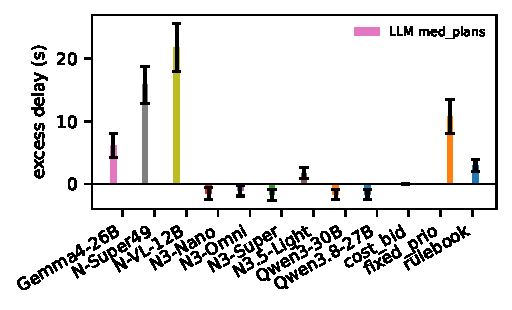
\includegraphics[width=\columnwidth]{fig/screen.pdf}
\caption{Model screen, mediator+plans arm, think=0 (200 paired encounters).
Negative excess beats the best-forced-yielder reference.}
\label{fig:screen}
\end{figure}
\begin{table}[t]\centering
\caption{Models screened (local vLLM on one GB10 node + hosted endpoint).}
\label{tab:models}
{\footnotesize\begin{tabular}{@{}lcc@{}}\toprule
Model & Params & Notes\\\midrule
Nemotron-3.5-Lightning & 30B-A3B & reasoning, MTP spec.\\
Nemotron-3-Nano & 30B-A3B & reasoning\\
Nemotron-3-Nano-Omni & 30B-A3B & reasoning, VL\\
Llama-3.3-Nemotron-Super & 49B & dense\\
Nemotron-Nano-VL & 12B & VL\\
Qwen3-30B-A3B & 30B-A3B & reasoning\\
Qwen3.8-27B & 27B & reasoning, VL\\
Gemma4-26B-A4B & 26B-A4B & VL\\
Muse-Glimmer & 30B & experimental\\
nemotron-3-super-120b (hosted) & 120B-A12B & NVIDIA API\\\bottomrule
\end{tabular}}
\end{table}
\subsection{Model screen}
Figure~\ref{fig:screen} screens all models on the mediator+plans arm (\texttt{think=0}). Reasoning mixture-of-experts models cluster tightly: qwen3.8-27B, qwen3-30B, and hosted nemotron-3-super reach $-1.7$\,s mean excess, nemotron-nano $-1.5$\,s, and nemotron-omni $-1.0$\,s --- all \emph{below} the forced-yielder reference (0.0\,s), because the reference picks the yielder but takes the planner's default refuge while the LLMs sometimes pick a better one. Right-yielder rates are 92--93\%. Nemotron-lightning underperforms (1.7\,s, 80\%) with 66\% parse fallback --- its traces frequently exhaust the 4096-token cap. The non-reasoning tier is starkly worse: gemma4-26B at 6.1\,s (75\%), dense nemotron-super-49B at 15.8\,s (42\%), and 12B nemotron-vl at 21.7\,s (38\%) --- worse than the hand-written rulebook (2.9\,s, 72\%) and approaching fixed priority (10.7\,s). A 1.5B smoke-test model collapsed entirely (25--47\,s, 25--30\% right). Deliberating $\sim$30B models thus meet or beat the benchmark's own reference; non-deliberating models do not negotiate, they guess.

\subsection{Deliberation is the capability}
\label{sec:think}
To test whether the reasoning trace carries the capability, we rerun the top models with \texttt{enable\_thinking=false} (verified empty reasoning fields, 9.3\,s to 4.2\,s mean call latency on qwen3.8). On identical encounters, qwen3.8-27B drops from $-1.7$\,s (93\% right) to $+11.1$\,s (66\%) on plans and $+23.2$\,s (40\%) on raw; qwen3-30B collapses further, to $+22.5$\,s (35\%) and $+29.9$\,s (36\%) --- below fixed priority and approaching the 1.5B failure mode (Fig.~\ref{fig:think}). The weights do not encode the corridor decision; the chain-of-thought computes it. Notably, even thinking-off agents receive identical plans numbers in the prompt --- they fail not for lack of the cost estimate but for lack of the arithmetic.
\begin{figure}[t]\centering
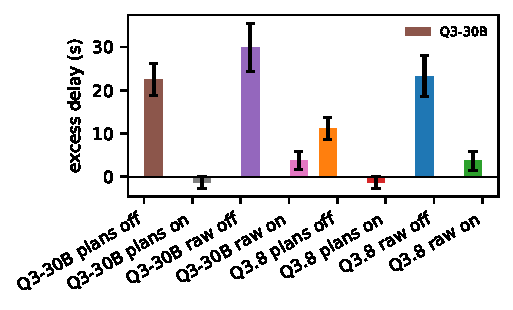
\includegraphics[width=\columnwidth]{fig/think.pdf}
\caption{Reasoning on vs off, mediator arms (paired seeds; on cells n=50).
Disabling chain-of-thought collapses decision quality.}
\label{fig:think}
\end{figure}
\begin{figure}[t]\centering
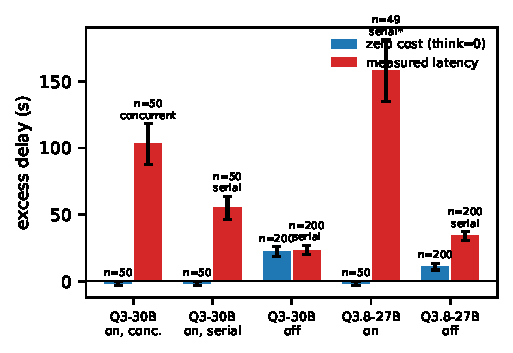
\includegraphics[width=\columnwidth]{fig/latency.pdf}
\caption{Quality-only vs measured-latency excess, mediator+plans. Charging real
inference time inverts the ranking; right-yielder is preserved.}
\label{fig:latency}
\end{figure}
\subsection{The deployed cost}
\label{sec:latency}
Decision quality is only half the story: a negotiator that takes 30--130\,s to answer stalls the robot mid-corridor. Charging measured latency as decision time inverts the ranking (Fig.~\ref{fig:latency}). qwen3-30B mediator+plans --- $-1.3$\,s in the quality arm --- rises to $+103.1$\,s excess with a 31.1\,s mean think, while \emph{right-yielder rate stays at 92\%}: the decisions are still correct, the robot simply pays for the deliberation in dead time. Worse, latency compounds into failure: on the raw arm, thinking-on+measured succeeds in only 64\% of encounters (88\% parse-fallback traces exceeding the token cap under pressure), leaving a third deadlocked. Thinking-off restores speed but not quality: a serial rerun gives 0.7\,s calls yet 23.6\,s excess --- latency is no longer the binding constraint, deliberation loss is. The deployed verdict is unambiguous: at current speeds, cost bidding (sub-millisecond, 0.0\,s) wins any real-time comparison; an LLM negotiator is viable only if deliberation is off the critical path --- precomputed, asynchronous, or sub-second.
% cost_bid wins deployed.
\subsection{Vision input}
\label{sec:vlm}
Four VL-capable models ran text-only, image-only (global render), and text+image mediator arms, thinking-off (Fig.~\ref{fig:vlm}). Image-only beats text-only on \emph{every} model --- gemma4 3.9 vs 6.6\,s, qwen3.8 9.0 vs 14.9\,s, nemotron-omni 14.2 vs 16.4\,s, vl-12b 17.0 vs 22.1\,s --- so visual grounding carries corridor geometry better than a numeric description for these models. Yet text+image is worse than image alone on three of four (e.g.\ vl-12b 30.0\,s, omni 20.6\,s): the modalities interfere rather than complement. All image arms still sit far below reasoning-on text ($-1$ to $-1.7$\,s) --- vision substitutes for deliberation only partially.
\begin{figure}[t]\centering
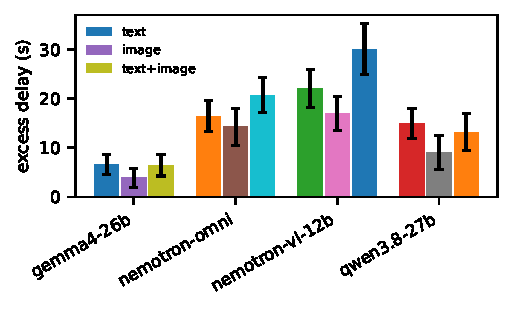
\includegraphics[width=\columnwidth]{fig/vlm.pdf}
\caption{Modality arms, mediator, thinking-off. Image-only beats text-only on
all four VL models; combining modalities interferes.}
\label{fig:vlm}
\end{figure}
\begin{figure}[t]\centering
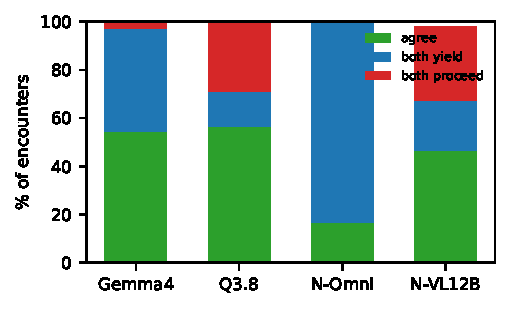
\includegraphics[width=\columnwidth]{fig/disagree.pdf}
\caption{Action-agreement modes, egocentric agents arm. Disagreement mode is a
model-specific personality: deference (both-yield) vs.\ self-serving conflict
(both-proceed).}
\label{fig:disagree}
\end{figure}

\subsection{Egocentric decentralized agents}
\label{sec:ego}
Chance encounters between unaffiliated robots motivate the agents mode: each robot gets only its egocentric view plus the peer's broadcast and decides independently. Here \emph{disagreement}, not decision quality, dominates --- and its mode is a model-specific personality (Fig.~\ref{fig:disagree}). nemotron-omni defers pathologically: both robots volunteer to yield on 84\% of encounters (deadlock-by-politeness, rulebook-rescued). qwen3.8-27B and vl-12b instead race ahead: both-proceed conflicts on 29\% and 31\% --- the reasons show self-serving attribution, each robot citing the \emph{same} proximity facts to award the yield to the \emph{other}. gemma4 is closest to healthy: 55\% agreement, mostly both-yield errors. On agreed encounters the right-yielder rate is only 58--71\%, and \emph{wrong-yielder agreements are the most expensive failure observed} (13.7--38.0\,s) --- correlated wrongness executes without any fallback. Ego images modestly beat raw text for weaker agents (vl-12b 5.3 vs 7.4\,s; qwen3.8 8.9 vs 10.0\,s) but cannot supply the coordination convention that is missing.
\subsection{The protocol default}
\label{sec:tiebreak}
Disagreement calls for a tiebreak --- but \emph{how} it is presented matters. We inject a fair, unspoofable draw: each robot's ``card'' is a hash bound to its id and the encounter time, computed identically from broadcast data, so neither can spoof it; the larger card wins on conflict. Three arms isolate presentation from resolution (Fig.~\ref{fig:tiebreak}).

\emph{Visible draw} (rule in the prompt): disagreements vanish entirely --- and so does deliberation. Agents preempt the draw rather than negotiate: right-yielder rate collapses to 48--58\% (coin-flip), and omni's trace shows it plainly --- ``A's card is smaller than B's, so if both yield or proceed, B would proceed.'' The common-knowledge default \emph{becomes} the policy.

\emph{Hidden draw} (identical prompts, draw resolves silently): answer distributions are \emph{identical} to the rulebook arm (e.g.\ omni 170/27/3 action-count split in both) --- deliberation is fully preserved. Conflicts now resolve by chance rather than optimally: 45--51\% right on tiebroken encounters, 11--14\,s excess, versus the rulebook's 99\% and 2--5\,s.

The triad separates incentive from mechanism: agent behavior tracks what they \emph{believe} the default is, not what it is --- and a fair default is only safe when it is worse than what agents can negotiate, or invisible.
\begin{figure}[t]\centering
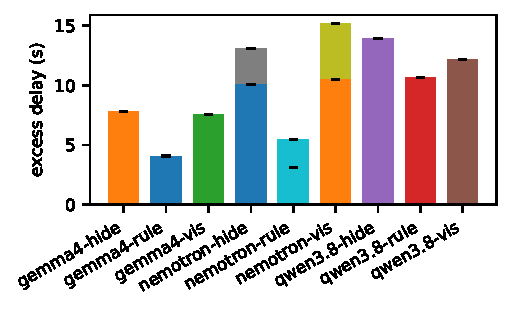
\includegraphics[width=\columnwidth]{fig/tiebreak.pdf}
\caption{Protocol-default triad: rulebook fallback vs hidden vs visible random
tiebreak (egocentric agents, paired seeds).}
\label{fig:tiebreak}
\end{figure}

\section{Discussion}
The picture that emerges is more optimistic than the latency numbers suggest --- and more cautionary than the quality numbers. For a fleet setting where a shared decision service is acceptable, a reasoning mediator with plans information is already at or beyond the benchmark's forced-yielder reference; the engineering work is making deliberation asynchronous (predictive negotiation, speculative caching of likely encounters, or a fast tier for routine cases). For true chance encounters between unaffiliated robots, decentralized foundation-model agents are not yet deployable: disagreement is structural, and a stated tiebreak fixes it only by destroying the reasoning that makes the agents useful. The practical guidance for protocol design is narrower than expected: keep defaults invisible, or make the negotiated outcome strictly better than the default --- a visible fallback is a policy, not a safety net.

\subsection{Limitations}
All results are simulation; the Gazebo transfer validated in~\cite{paper1} covers classical policies, not the LLM arms. Two layouts and one encounter type bound the generality. The hosted 120B endpoint was unreliable under study load ($\sim$100\% errors on several cells), so its screen number is the only trusted hosted datapoint. Thinking-off is honored on the models tested but is not universal across serving stacks, and several models' traces exceed the 4096-token cap on the raw prompt (the parse-fallback counts reflect this). Finally, agents answer a single-shot prompt; multi-turn dialogue, tool use (querying the planner), and selfish-utility prompts are untested arms.

\section{Conclusion}
Reasoning-capable language models \emph{can} negotiate head-on robot encounters at or beyond a strong classical reference --- the capability is real, and it is the deliberation, not the parameters. But deployed viability is governed by latency, not decision quality: at current inference speeds a millisecond bid mechanism wins by an order of magnitude. For decentralized agents, coordination conventions --- not perception --- are the bottleneck: models disagree in personality-specific ways that better sensing does not fix. And the mechanism-design lesson generalizes: for LLM agents, the stated default is not a floor but a magnet. Design protocols accordingly.

\bibliographystyle{IEEEtran}
\bibliography{refs}
\end{document}
